% Lecture for ph2a Caltech 2017: Vibrations and Waves
\documentclass[pdf,hideothersubsections]{beamer}
\usepackage{beamerthemeshadow}
\mode<presentation>
  {
    \usefonttheme{structuresmallcapsserif}
    \usetheme{PaloAlto}
    \usecolortheme{seagull}
    %\useinnertheme{circles}
%    \useoutertheme{tree}
  }

\usepackage{svg}
\usepackage{xmpmulti}

\usepackage{hyperref}
\hypersetup{
    pdffitwindow=true,     % window fit to page when opened
    colorlinks=true,       % false: boxed links; true: colored links
    linkcolor=orange,          % color of internal links (change box color with linkbordercolor)
    citecolor=green,        % color of links to bibliography
    filecolor=magenta,      % color of file links
    urlcolor=blue           % color of external links
}

% Fonts/encoding
\renewcommand{\UrlFont}{\tiny}
\usepackage[utf8]{inputenc}
\usepackage[T1]{fontenc}
%\usepackage[sc,medium,raggedright]{titlesec}
\usepackage{newtxmath}
%\usepackage{libertine}
\usepackage[osf]{ebgaramond}

\graphicspath{{Figures/}}

\begin{document}
\title{Superposition}  
\author{Caltech: ph2a}
\date{28 - Sep - 2017}
%\logo{
\includegraphics[height=0.5cm]{../caltech_logo.png}}

\frame{\titlepage} 

\frame{\frametitle{Table of contents}\tableofcontents} 

\section{Previous Summary}
\begin{frame}
\frametitle{Tuesday}
\begin{itemize}
\item Many physical systems involving small vibrations can be represented as a Simple Harmonic Oscillator.

\item Complex exponentials can be used to solve oscillator problems.

\item Guess solutions; set constants by setting (Dirichlet, Neumann, Cauchy) boundary conditions.

\item Imaginary part of the complex frequency corresponds to damping.
\end{itemize}
\end{frame}


\section{Damped Electrical Circuit}
\begin{frame}
\frametitle{Complex approach to damped SHO}
Use the same approach as before:
\begin{itemize}
\item $L \ddot{Q} + R \dot{Q} + Q/C = 0$
\pause
\item $\tilde{Q}(t) = A e^{i (\omega t + \phi_0)}$
\pause
\item $-L \omega^2 \tilde{Q} + i \omega R \tilde{Q} + \tilde{Q}/C = 0$
\end{itemize}
\pause
Dividing by $L \tilde{Q}$, we get a quadratic equation for $\omega$: \\
\pause
\begin{center}
$\omega = \sqrt{\omega_0^2 - \Big(\frac{R}{2 L}\Big)^2} + i \frac{R}{2 L}$ \\
\end{center}
\pause
Let's call the real part $\omega$ and plug back into the guess for x(t):
\pause
\begin{center}
$\tilde{x} = A e^{i (\omega t + \phi_0)} e^{-(R/2 L) t}$\\
\end{center}
\pause
We can define the time constant: $\tau \equiv 2 L/R$, so that: \\
\pause
Taking the real part, we find the solution as before (with the damping): \\
\pause
\begin{center}
$Re\left\{\tilde{Q}\right\} = Q = A \cos(\omega t + \phi_o) e^{-t/\tau}$
\end{center}

\end{frame}


\begin{frame}
\frametitle{Decaying Oscillation}

\centering
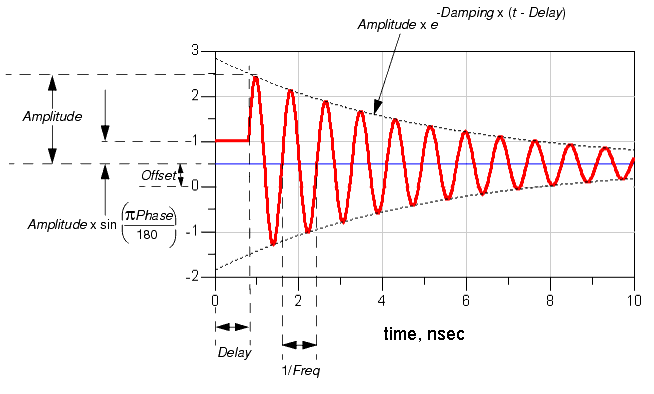
\includegraphics[width=\textwidth]{damped_sine.png}

\end{frame}


\subsection{Damped Oscillations of a Black Hole}
\begin{frame}
\frametitle{Black Hole Vibrations: Yesterday's Press Release}
\centering
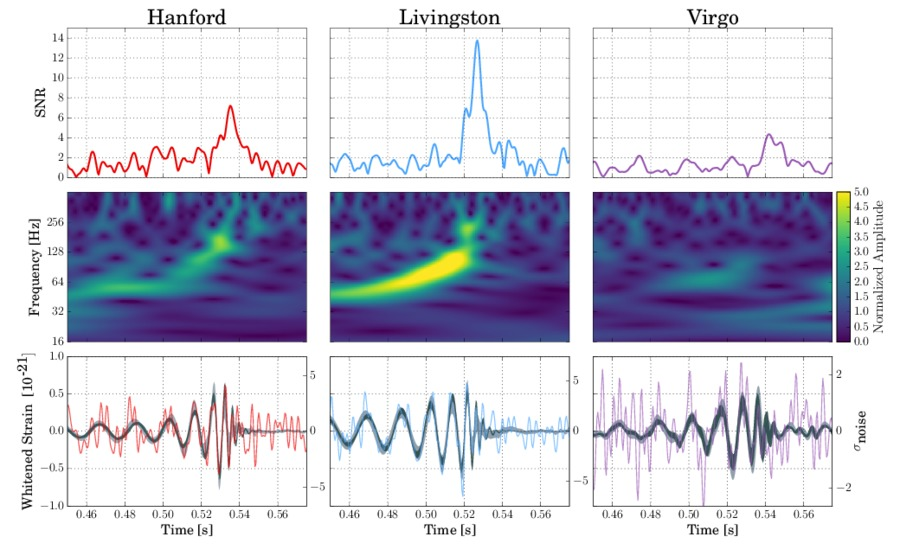
\includegraphics[width=\textwidth]{GW170814-TF.jpg}

\begin{itemize}
   \item \url{https://www.ligo.caltech.edu/video/ligo20160211v10}
   %\item \url{http://demonstrations.wolfram.com/DrivenDampedOscillator/}
   %\item \url{http://demonstrations.wolfram.com/SimpleHarmonicMotionForASpring/}
\end{itemize}
\end{frame}


\subsection{Applying Boundary Conditions}

\frame{\frametitle{Boundary Conditions}
In both cases, there are two free constants (A \& B, or D \& $\phi_0$). \\
\pause
These constants are set to force the solution to match any 'Boundary' conditions: \pause
\begin{itemize}
\item initial displacement \pause
\item initial velocity \pause
\item e.g., mass is released at t=0 with x = x$_0$
\end{itemize}

}

\frame{\frametitle{Boundary Conditions: Example}



}

\section{Sum of Vibrations}
\begin{frame}
\frametitle{Adding sinusoids}
Addition of two sinusoidal signals can be handled by vector addition of complex \emph{phasors}.
\pause
\begin{columns}[T]
  \begin{column}{0.5\textwidth}
    \begin{centering}
      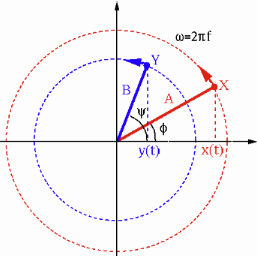
\includegraphics[width=4cm]{RotatingVectors2.png}
    \end{centering}
  \end{column}
  \pause
  \begin{column}{0.5\textwidth}
    \begin{centering}
      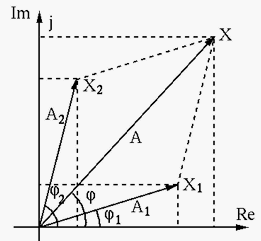
\includegraphics[width=4cm]{phasoraddition1a.png}
    \end{centering}
  \end{column}

\end{columns}

\end{frame}

\subsection{Two Vibrations}
\begin{frame}
\frametitle{Two Sine Waves}

\begin{itemize}
\item Different Phases (demo)
\item Different Frequencies (demo)
\end{itemize}

\end{frame}
%\subsection{Many vibrations with random phase}

%\subsection{Acoustic Beats}


\section{The Pendulum}
\begin{frame}
\frametitle{Pendula}

\begin{columns}[T]
   \begin{column}{0.5\textwidth}
    The LIGO detectors which were used to detect those black hole signals, use lasers and mirrors\footnotemark to detect those tiny vibrations in the space-time continuum. To isolate the mirrors from the ground motion, the mirrors are hung with 
glass fibers as pendula\footnotemark.

   \end{column}

   \pause
   \begin{column}{0.5\textwidth}
   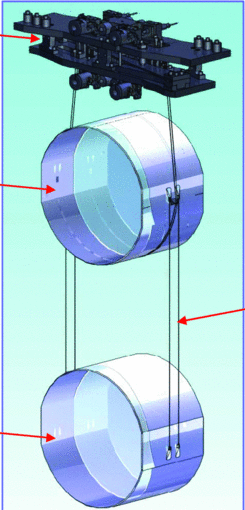
\includegraphics[height=6cm]{LIGO-Pendulum-diagram.png}      

   %\pause
   %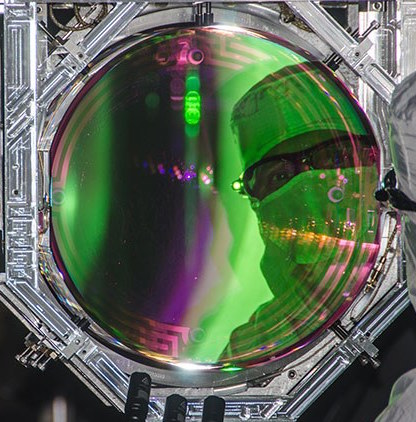
\includegraphics[height=4cm]{LIGO-Mirror.jpg}      
   \end{column}
  
\end{columns}
\footnotetext[1]{\url{https://www.ligo.caltech.edu/video/ligo20170216v}}
 \footnotetext[2]{\url{https://www.khanacademy.org/science/physics/mechanical-waves-and-sound/harmonic-motion/v/pendulum}}

\end{frame}

\begin{frame}
\frametitle{Pendula}

\begin{columns}[T]
   \begin{column}{0.5\textwidth}
    The LIGO detectors which were used to detect those black hole signals, use lasers and mirrors\footnotemark 
to detect those tiny vibrations in the space-time continuum. To isolate the mirrors from the ground motion, the mirrors are hung with 
glass fibers as pendula\footnotemark.

   \end{column}

   \pause
   \begin{column}{0.5\textwidth}
   %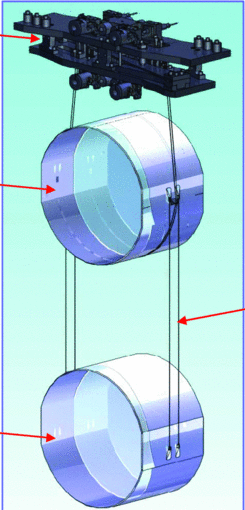
\includegraphics[height=6cm]{LIGO-Pendulum-diagram.png}      

   %\pause
   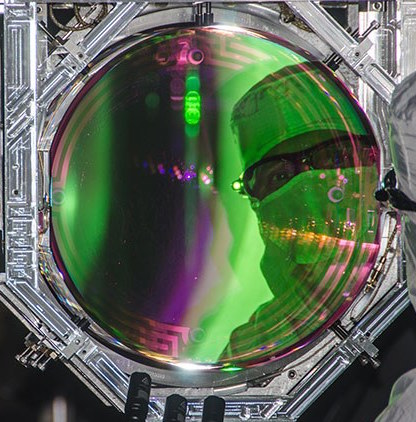
\includegraphics[height=4cm]{LIGO-Mirror.jpg}      
   \end{column}
  
\end{columns}
\footnotetext[1]{\url{https://www.ligo.caltech.edu/video/ligo20170216v}}
 \footnotetext[2]{\url{https://www.khanacademy.org/science/physics/mechanical-waves-and-sound/harmonic-motion/v/pendulum}}

\end{frame}

\subsection{Analysis}
\begin{frame}
\frametitle{Construct the Diff. Eq.}
\begin{columns}[T]

  \begin{column}{0.3\textwidth}
     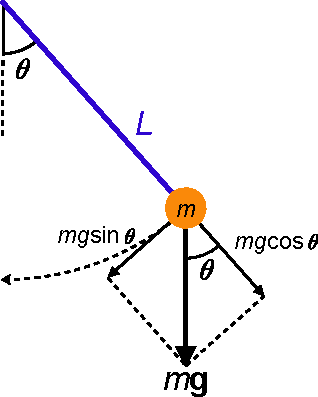
\includegraphics[width=\textwidth]{Simple_pendulum_generalized_coordinates.pdf}

  \end{column}
\pause
  \begin{column}{0.7\textwidth}
  \begin{enumerate}
  \item Motion of pendulum is \emph{rotational}, not translational, so instead of $F = m a$, use $\tau = I \ddot{\theta}$, where $\tau$ is the torque, and $\theta$ is the angle of the pendulum wire. \\
    \pause
  \item In the case of a point mass rotating around an origin, $I = m r^2$. \\
    \pause
  \item The torque is the cross product of the Force and the lever arm: $\vec{\tau} = \vec{r} \times \vec{F}$, so: \\
  \end{enumerate}
  \pause
  \begin{align*}
I \ddot{\theta} &= \vec{r} \times \vec{F} \\
m L^2 \ddot{\theta} &= -m g L \sin{\theta} \\
\ddot{\theta} &= -\frac{g}{L} \sin{\theta} \\
  \end{align*}
  %\pause
  %Ugh - sine is not a linear function...
  \end{column}

\end{columns}

\end{frame}
\subsection{Simulation}
\begin{frame}
\frametitle{Numerically Solve the Pendulum Problem}
\begin{itemize}
\item $\ddot{\theta} = -\frac{g}{L} \sin{\theta}$
\pause
\item $\dot{\theta} = \int_{t_1}^{t_1 + \delta t} \ddot{\theta}(u) du $
\pause
\item $\theta = \int_{t_1}^{t_1 + \delta t} \dot{\theta}(u) du $
\pause
\item Interactive Demo: \url{https://phet.colorado.edu/en/simulation/pendulum-lab}
\end{itemize}
\end{frame}

\subsection{Linearized Solution}
\begin{frame}
\frametitle{Linearizing the Pendulum: I}
\begin{itemize}
\item In many physical situations (not just black holes), the restoring force is not linear; i.e. the potential energy is not just quadratic.
\pause
\item Luckily, many interesting and useful analyses can be done by linearization:
\pause
\item Assume that: (1) The potential exists, (2) We're analyzing the equilibrium position, and (3) we care only about small motions around equilibrium.
\end{itemize}
\pause

\begin{block}{Taylor Series expansion: Ch.1 (Eq. 1-9)} 
$V(x) = V(0) + V'(0) x + \frac{1}{2} V''(0) x^2 + \ldots$
\end{block}
\pause

Equilibrium $\Rrightarrow V'(0) = 0$, \& $F = -\frac{dV}{dx}$, so...
\pause
$F = - k_{eff} x$

\end{frame}


\begin{frame}
\frametitle{Linearizing the Pendulum: II}
Equation for the frictionless pendulum:
\begin{align*}
\onslide<1->{\ddot{\theta} &= -\frac{g}{L} \sin{\theta} \\}
\onslide<2->{  &\simeq -\frac{g}{L} \Big[\theta - \frac{\theta^3}{3 !} + \ldots \Big] \\}
\onslide<3->{  &\simeq -\frac{g}{L} \theta}
\end{align*}
\onslide<4-> {Which has the same form as SHO equation for the mass-spring and RLC systems and so, as before, $\tilde{\theta} = A e^{i (\omega t + \phi_0)}$}

\end{frame}

\section{Summary}
\begin{frame}
\frametitle{Summary}
\begin{enumerate}
\item For linear systems, the resultant of two vibrations is just their sum.
\pause
\item Summation of two oscillations with same period but different phase can be solved by vector addition of their complex phasors.
\pause
\item Sum of two oscillations with different frequencies leads to \emph{beats}.
\pause
\item Many non-linear systems can be analyzed by linearization.
\pause
\item Beating is apparent in physical systems even without non-linearity.
\end{enumerate}
\end{frame}


\end{document}

